\documentclass[oneside]{article}

\usepackage[english]{babel}

\usepackage[a4paper,top=2cm,bottom=2cm,left=2cm,right=2cm,marginparwidth=1.75cm]{geometry}
\usepackage{fancyhdr}
\pagestyle{fancy}

% Useful packages
\usepackage[shortlabels]{enumitem}
\usepackage{enumitem}
\usepackage{amsmath}
\usepackage{bbold}
\usepackage{graphicx}

\usepackage{bbm}
\usepackage{mathrsfs}
\usepackage{graphicx}
\usepackage{epstopdf}
\usepackage[colorlinks=true, allcolors=blue]{hyperref}
\usepackage{lmodern}
\usepackage[T1]{fontenc}
\usepackage[utf8]{inputenc}
\usepackage{textcomp}
\usepackage{matlab-prettifier}
\usepackage{blindtext}
\usepackage{float}
\usepackage{url}
\usepackage{multirow}
\usepackage{subcaption}

% automatic EPS conversion 
\usepackage{graphicx} 
\usepackage{epstopdf}

\fancyhf{}
\usepackage{titling}
\setlength{\headheight}{35pt}
\addtolength{\topmargin}{-10pt}
\fancyhf[HC]{\thetitle}
\fancyhf[HR]{\theauthor}
\fancyhf[HL]{\today}
\fancyhf[FR]{\thepage}

\title{Report for Assignment 1\\Course DAT600-1 25V Algorithm Theory}
% Insert your names
\author{Filip Dasek\\--Ali--\\--Cipher--}
\date{\today}

\begin{document}

\maketitle
\pagenumbering{gobble}
\newpage
\pagenumbering{arabic}

\section{Recording of the complexity of sorting algorithms}

\begin{figure}[H]
    \centering
    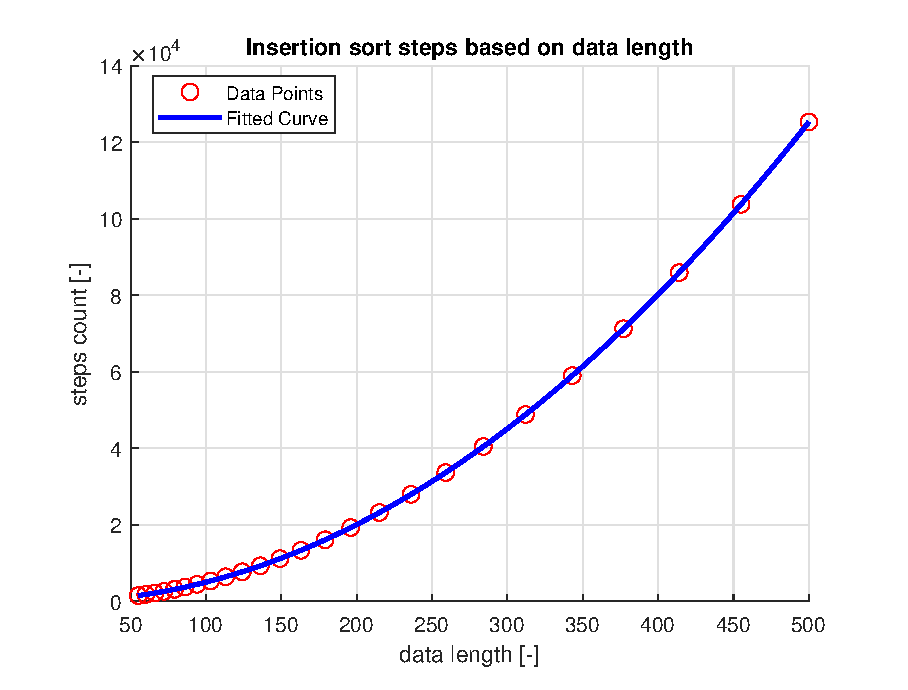
\includegraphics[width = 0.8\textwidth]{is_count_figure.eps}
    \caption{Insertion sort complexity graph}
    \label{fig:is_count}
\end{figure}

\begin{figure}[H]
    \centering
    \includegraphics[width = 0.8\textwidth]{ms_count_figure.eps}
    \caption{Merge sort complexity graph}
    \label{fig:ms_count}
\end{figure}

\begin{figure}[H]
    \centering
    \includegraphics[width = 0.8\textwidth]{hs_count_figure.eps}
    \caption{Heap sort complexity graph}
    \label{fig:hs_count}
\end{figure}

\begin{figure}[H]
    \centering
    \includegraphics[width = 0.8\textwidth]{qs_count_figure.eps}
    \caption{Quick sort complexity graph}
    \label{fig:qs_count}
\end{figure}




\end{document}

